\documentclass[10pt, journal]{IEEEtran}
\usepackage{amsmath}
\usepackage{amsfonts}
\usepackage{amssymb}
\usepackage{hyperref}
\usepackage{graphicx}
\graphicspath{ {images/} }
\usepackage[caption=false,font=footnotesize]{subfig}
\usepackage{siunitx}

\title{Figures}

\newcommand{\norm}[1]{\left\lVert#1\right\rVert}

\begin{document}
\maketitle

\begin{figure*}
  \centering
  \subfloat[]{
    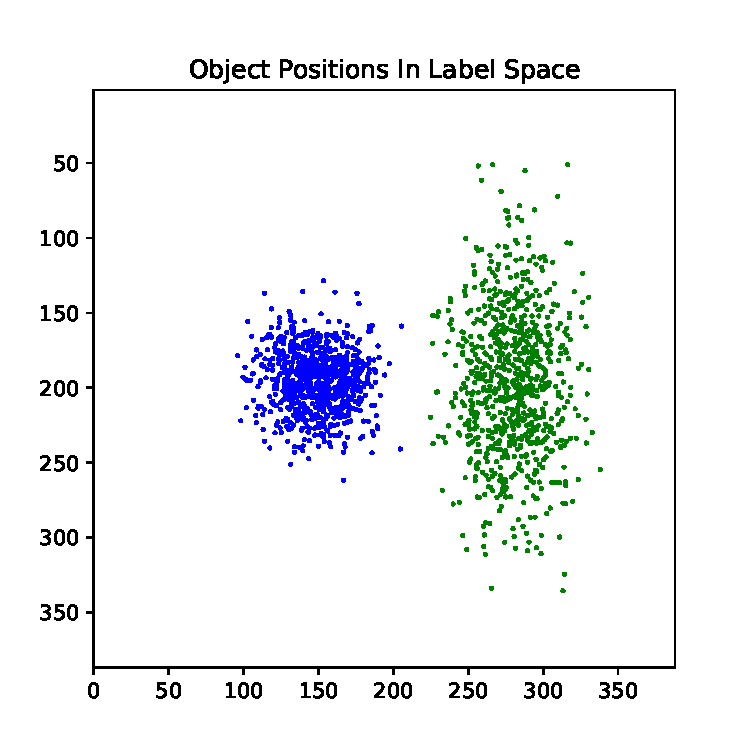
\includegraphics[width=0.49\linewidth]{object_positions_in_label_space}
    \label{fig:object-positions-in-label-space}
  }
  \subfloat[]{
    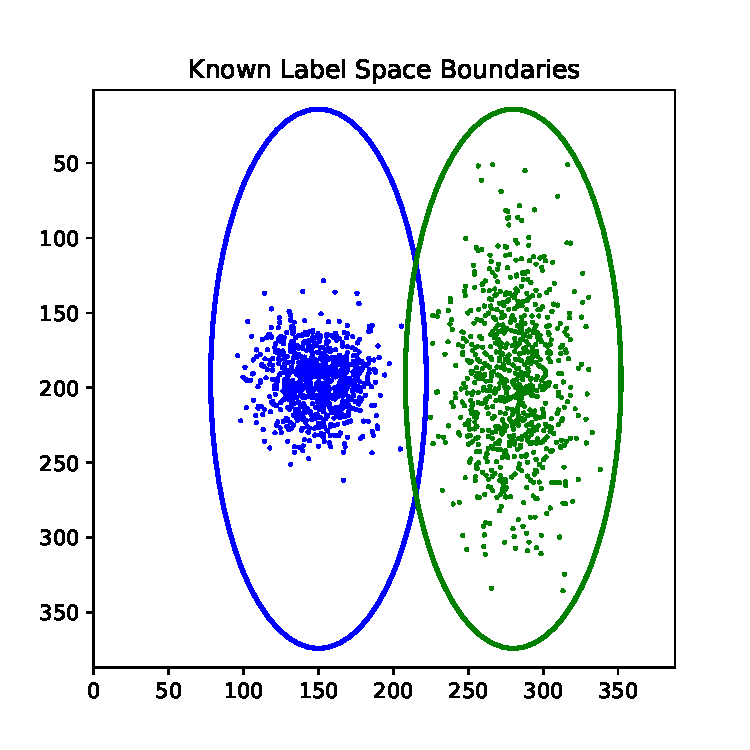
\includegraphics[width=0.49\linewidth]{known_label_space_boundaries}
    \label{fig:known-label-space-boundaries}
  } \\
  \subfloat[]{
    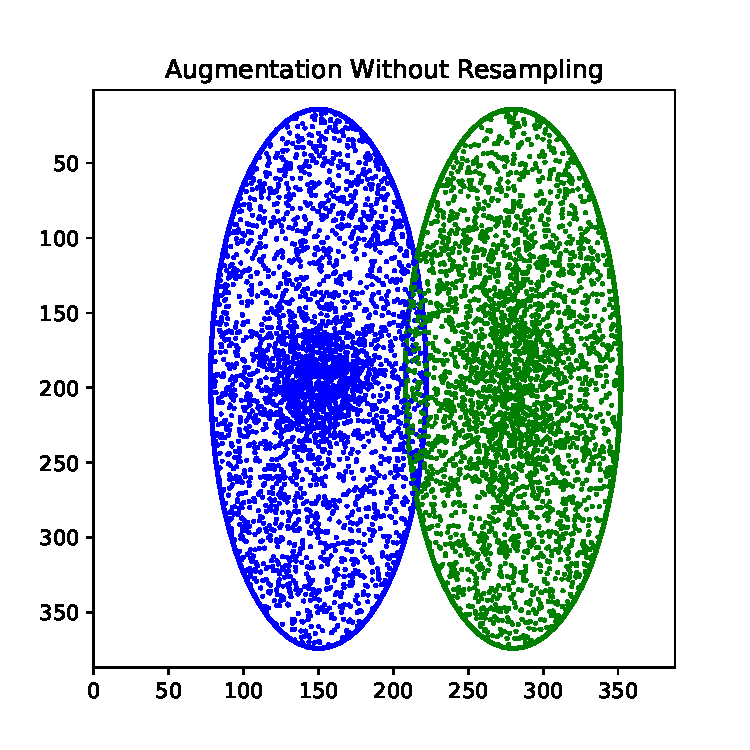
\includegraphics[width=0.49\linewidth]{augmentation_without_resampling}
    \label{fig:augmentation-without-resampling}
  }
  \subfloat[]{
    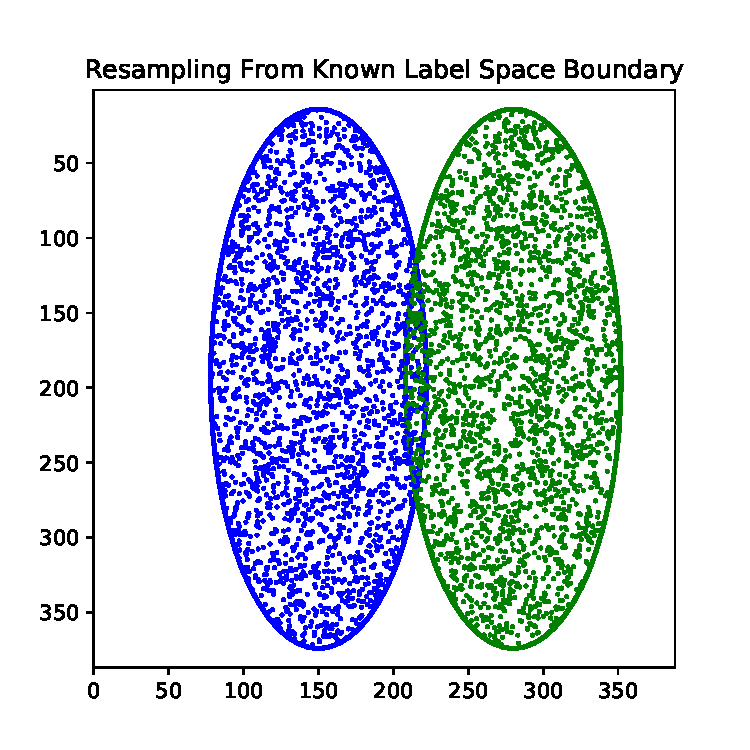
\includegraphics[width=0.49\linewidth]
    {resampling_from_known_label_space_boundary}
    \label{fig:resampling-from-known-label-space-boundary}
  }
  \caption{For any experiment, object positions in label-space will have some
    natural distribution evident in the original dataset, such as in
    (\ref{fig:object-positions-in-label-space}). Generally, an experimenter
    knows absolute boundaries for each object's distribution, such as in
    (\ref{fig:known-label-space-boundaries}), because she imposes them during
    collection. To analyze object positions (or other properties) in an unbiased
    way, a Deep Neural Network (DNN) should be trained on images corresponding
    to labels from within that
    boundary. (\ref{fig:augmentation-without-resampling}) shows how one might
    select new points in label-space to generate images for, keeping all the
    original points. (\ref{fig:resampling-from-known-label-space-boundary})
    shows a resampling that keeps original points only within the desired
    distribution, preventing dataset bias.}
  \label{fig:label-space}
\end{figure*}

\begin{figure*}
  \centering
  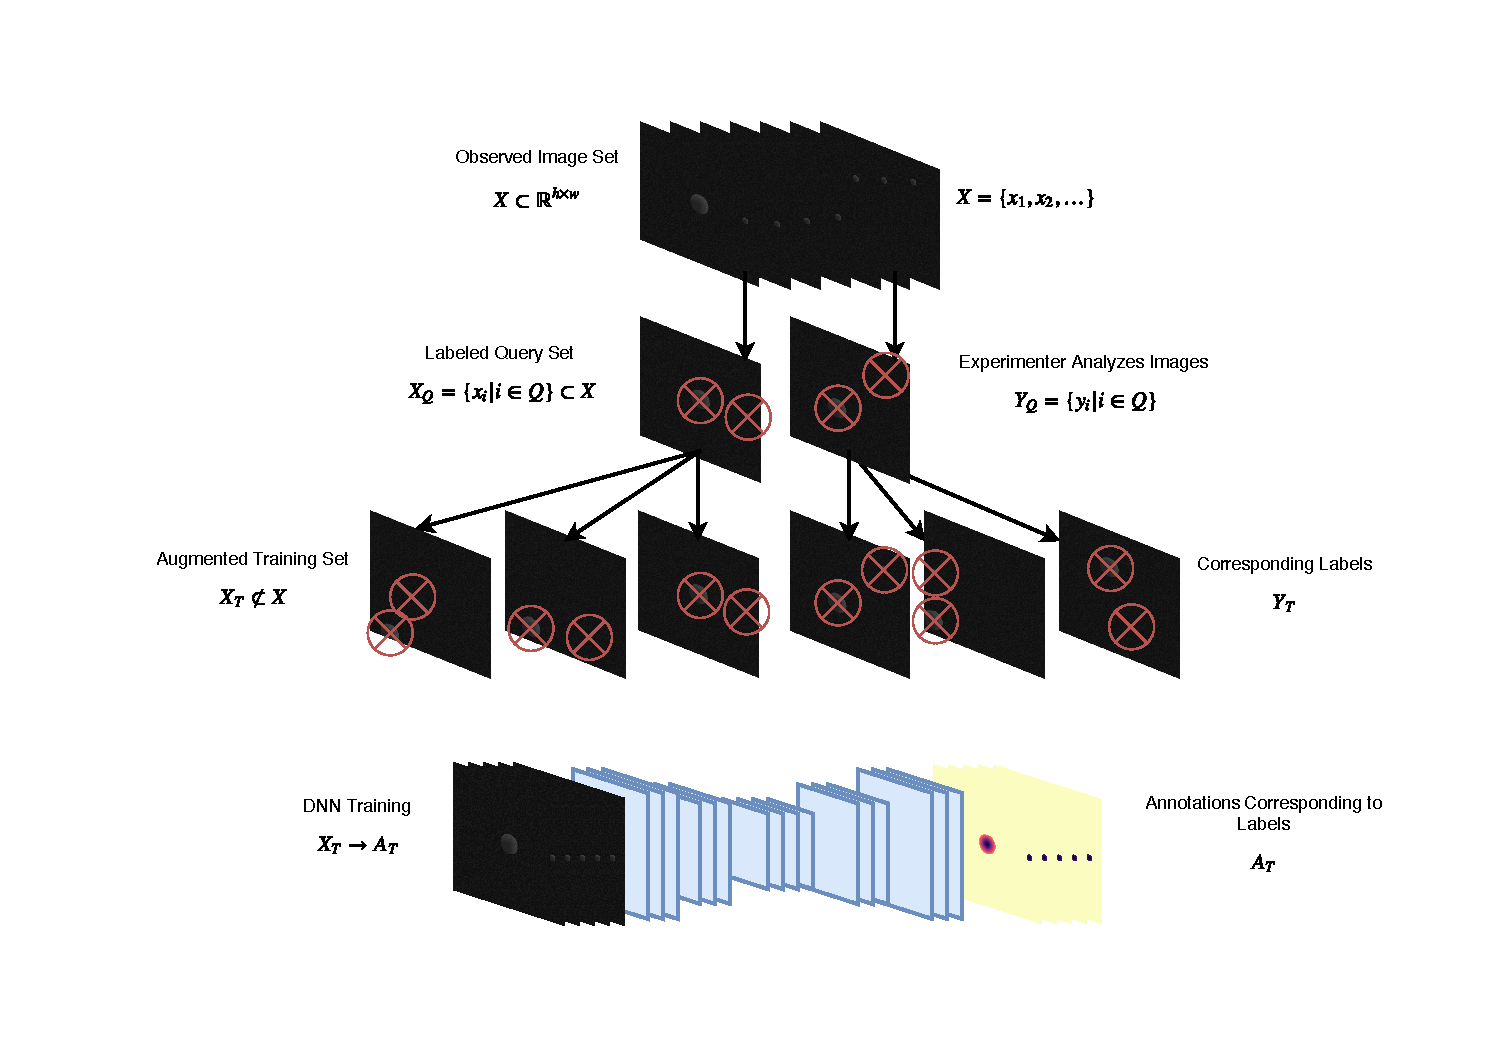
\includegraphics[width=\linewidth]{training}
  \caption{Given original images observed during experiment time
    $X \in \mathbb{R}^{h\times w}$, a DNN-facilitated method for image analysis
    aims to minimize the analysis provided by an experimenter. Therefore, we
    select a query set $X_Q$ of images that will most facilitate learning. For
    each of these images, the experimenter provides analysis which consists of
    labels $y_i$ for each image (shown in red). In order to create training
    images $X_T$, we add new images by transforming elements of $X_Q$. For
    instance, we might translate image objects corresponding with new points in
    label-space, obtained as in Fig. (\ref{fig:label-space}). Training
    annotations $A_T$ are obtained from $Y_T$ according to Eq. (\ref{eq:1}),
    after which we train the object detection DNN on $(X_T, A_T)$.}
  \label{fig:training}
\end{figure*}

An annotation $a \in \mathbb{R}^{h\times w}$ for object positions corresponds to
a labeling of object positions $y \in \mathbb{R}^{n\times 2}$, where $n$ is the
number of objects in the image. If $y_k \in \mathbb{R}^2$ is the position of
object $k$ in the image, then we can obtain the annotation according to
\begin{equation}
  \label{eq:1}
  a_{ij} = \min\left(D_{\max},
    \min_k \norm{
      \begin{bmatrix}
        i \\
        j
      \end{bmatrix} - y_k}^2
  \right)
\end{equation}
where $D_{\max}$ is a maximum distance threshold.
 

\end{document}
%%% Local Variables:
%%% mode: latex
%%% TeX-master: t
%%% End:
